\documentclass{paper}
\usepackage{authblk}
\usepackage{graphicx}
\usepackage{wrapfig}
\usepackage{cite}
\usepackage[margin=1.0in]{geometry}

\title{Blowship}
\author[*]{John Carlyle}
\author[**]{Morgan McDermott}
\affil[*]{University of fighitng bears}
\affil[**]{University of sillypants}

\begin{document}
\maketitle
\twocolumn
\section{Introduction}
Lorem ipsum dolor sit amet, consectetur adipisicing elit, sed do eiusmod tempor incididunt ut labore et dolore magna aliqua. Ut enim ad minim veniam, quis nostrud exercitation ullamco laboris nisi ut aliquip ex ea commodo consequat. Duis aute irure dolor in reprehenderit in voluptate velit esse cillum dolore eu fugiat nulla pariatur. Excepteur sint occaecat cupidatat non proident, sunt in culpa qui officia deserunt mollit anim id est laborum.Lorem ipsum dolor sit amet, consectetur adipisicing elit, sed do eiusmod tempor incididunt ut labore et dolore magna aliqua. Ut enim ad minim veniam, quis nostrud exercitation ullamco laboris nisi ut aliquip ex ea commodo consequat. Duis aute irure dolor in reprehenderit in voluptate velit esse cillum dolore eu fugiat nulla pariatur. Excepteur sint occaecat cupidatat non proident, sunt in culpa qui officia deserunt mollit anim id est laborum.Lorem ipsum dolor sit amet, consectetur adipisicing elit, sed do eiusmod tempor incididunt ut labore et dolore magna aliqua. Ut enim ad minim veniam, quis nostrud exercitation ullamco laboris nisi ut aliquip ex ea commodo consequat. Duis aute irure dolor in reprehenderit in voluptate velit esse cillum dolore eu fugiat nulla pariatur. Excepteur sint occaecat cupidatat non proident, sunt in culpa qui officia deserunt mollit anim id est laborum.Lorem ipsum dolor sit amet, consectetur adipisicing elit, sed do eiusmod tempor incididunt ut labore et dolore magna aliqua. Ut enim ad minim veniam, quis nostrud exercitation ullamco laboris nisi ut aliquip ex ea commodo consequat. Duis aute irure dolor in reprehenderit in voluptate velit esse cillum dolore eu fugiat nulla pariatur. Excepteur sint occaecat cupidatat non proident, sunt in culpa qui officia deserunt mollit anim id est laborum.Lorem ipsum dolor sit amet, consectetur adipisicing elit, sed do eiusmod tempor incididunt ut labore et dolore magna aliqua. Ut enim ad minim veniam, quis nostrud exercitation ullamco laboris nisi ut aliquip ex ea commodo consequat. Duis aute irure dolor in reprehenderit in voluptate velit esse cillum dolore eu fugiat nulla pariatur. Excepteur sint occaecat cupidatat non proident, sunt in culpa qui officia deserunt mollit anim id est laborum.Lorem ipsum dolor sit amet, consectetur adipisicing elit, sed do eiusmod tempor incididunt ut labore et dolore magna aliqua. Ut enim ad minim veniam, quis nostrud exercitation ullamco laboris nisi ut aliquip ex ea commodo consequat. Duis aute irure dolor in reprehenderit in voluptate velit esse cillum dolore eu fugiat nulla pariatur. Excepteur sint occaecat cupidatat non proident, sunt in culpa qui officia deserunt mollit anim id est laborum.Lorem ipsum dolor sit amet, consectetur adipisicing elit, sed do eiusmod tempor incididunt ut labore et dolore magna aliqua. Ut enim ad minim veniam, quis nostrud exercitation ullamco laboris nisi ut aliquip ex ea commodo consequat. Duis aute irure dolor in reprehenderit in voluptate velit esse cillum dolore eu fugiat nulla pariatur. Excepteur sint occaecat cupidatat non proident, sunt in culpa qui officia deserunt mollit anim id est laborum.Lorem ipsum dolor sit amet, consectetur adipisicing elit, sed do eiusmod tempor incididunt ut non proident, sunt in culpa qui officia deserunt mollit anim id est laborum.Lorem ipsum dolor sit amet, consectetur adipisicing elit, sed do eiusmod tempor incididunt ut non proident, sunt in culpa qui officia deserunt mollit anim id est laborum.Lorem ipsum dolor sit amet, consectetur adipisicing elit, sed do eiusmod tempor incididunt ut
\section{Previous Work}
There has been a plethora of original work and refinement in the area of anonymous internet communication. Broadly categorized, these include:
\begin{enumerate}
  \item Mixes \cite{chaum-mix} 
  \item Onion routing \cite{onion-discex00}
  \item Freedom (wtf) [z]
\end{enumerate}
\section{Privacy Goals}
  The goal of this system is to provide an in-browser method for communicating securely between parties without massive latency or communication overhead. We attempt to satisfy these requirements assuming the intermediate server may be compromised. By communicating securely we mean specifically (using terminology from \textbf{[6]}):
  \\\\\textbf{Communication Privacy}. Any party Eve cannot read the contents of intercepted messages sent between any two parties Alice and Bob. 
  \\\textbf{Participant Privacy}. This is also called \textbf{Unobservability} and \textbf{Untraceability}. Any party Eve, cannot determine with probability $p > \epsilon$ that the two are communicating, given any $\epsilon$ chosen by Alice and Bob (with a clear lower bound of $\epsilon > 1/N$ where $N$ is the number of participants). The ability of multiple participants to collude and determine this with $p > \epsilon$ must be well defined.
  \\\textbf{Destination Privacy}. Any party Eve in the network cannot determine the final destination of any party Alice's messages. This is a less stringent requirement than Participant Privacy.
\section{PSP}
In this section we introduce
$P2(S2P2)^nP$, or PSP for short. PSP is an alternative to P2P protocols in which peers communicate with eachother through an alternating chain of peer-server and server-peer communications.

\begin{figure}[ht]
  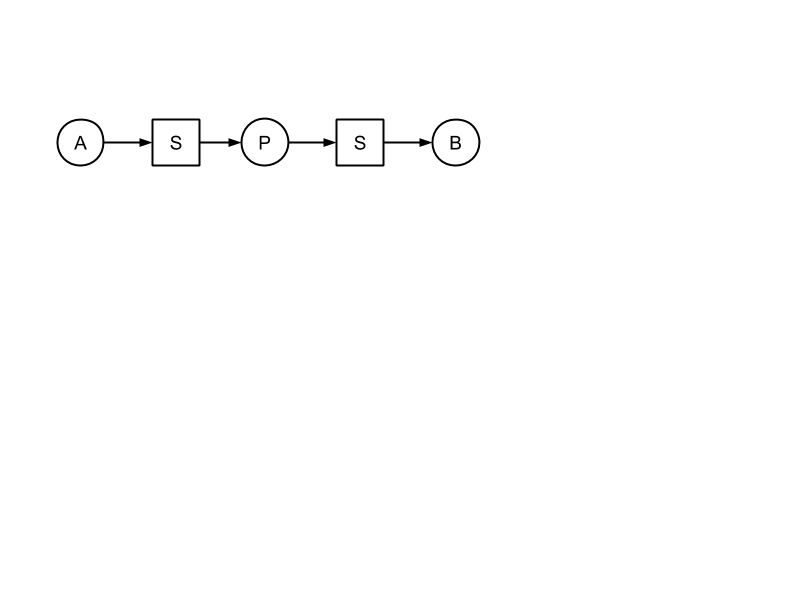
\includegraphics[width=230px]{PSP.png}
  \caption{A simple PSP communication chain}
\end{figure}

\subsection{Basic Protocol}
Assume that Alice has obtained Bob's public key and unique ID while maintaining her anonymity. Assume also that Alice can obtain the public keys and IDs for $n \le N$ peers at random while hiding her choice from Surge. 

Alice can then send a message to bob that will follow the path $A \rightarrow P_1 \rightarrow S \rightarrow ... \rightarrow S \rightarrow P_n \rightarrow B$ by sending the following message to Surge: 
\\
Let $M = E_{KRA}[  time || nonce || message ]$
\\Let $F_{ij}[x] = E_{KUi}[ ID_j || E_{KUj}[ x ] ]$
\\
Alice sends: $F_{S1}[F_{S2}[...F_{nB}[ M ]]]$ to Surge. 

Each successive party receives a message and an ID to forward that message to, and only that party can read its message. Importantly, any Penguin or Proletariat without collusion from Surge doesn't gain any information about the source or destination of the message it's passing along. 

Note that Surge can't track a message by its contents, since it gets decrypted and changed by each successive peer. 

In this system, peers operate exactly as MIXes in the literature \cite{chaum-mix} . That is, they prevent traffic correlation by removing a layer of encryption, prevent relay attacks [[[TODO]]], as well (as we will discuss) by reordering and batching messages. 
\subsection{Adversaries}
In this context, we have several distinct types of adversaries we must consider:
\begin{enumerate}
  \item\textbf{Penguin.} Penguin is any Peer who can intercept and alter messages being passed through it. 
  \item\textbf{Surge.} Surge is a compromised central Server. He can alter and intercept any messages passing through, and can provide bogus information to any peer.
  \item\textbf{Proletariat.} The Proletariat is a group of colluding Penguins.
  \item\textbf{The Palace.} The Palace is a collusion of the Proletariat and Surge.
\end{enumerate}
\subsection{Security Flaws}
Here we'll perform a simplified analysis of the security flaws of the basic, naive system described so far. 
Let $P_{AB}$ be the probability that Alice is talking to Bob. 
\begin{enumerate}
\item\textbf{Linear Chain.} If we assume that Alice's message is the only message sent by any of $P_1 ... P_n$, $Surge$ can determine that $P_{AB} > (n+1)^{-1} \gg 1/N$. This is because Surge knows that one of $A \cup \{P_1 ... P_n\}$ talked to Bob.
\item\textbf{Collusion.} If there is a Proletariat of size $s$ colluding with Surge to form the Palace, then the Palace can determine on average (depending on which peers Alice picked), that $P_{AB} > (n/(N-s)+1)^{-1}$ - that is, Alice has a chance $1 - (N-s)/N$ of each peer being compromised and not contributing to her privacy.
\item\textbf{Timing.} Even if $P_1 ... P_n$ are sending other messages, if Surge knows the probability distribution of the peer delay between receiving a message and forwarding it, he can discover the increased probability that Alice and Bob are talking. 
\item\textbf{Multiple Communications.} If Alice sends another message to Bob, or Bob back to Alice, the chance that they are communicating increases even more. 
\end{enumerate}
This is fairly poor security. If Alice chooses $n = 5$, then if her chosen peers send no other messages until hers is delivered, Surge knows $P_{AB} > 1/6$ chance that Alice is talking to Bob. If $60\%$ of peers are part of the Palace, then Surge possibly knows $P_{AB} = 1$ if $n \subset s$, but the expectation is $E[P_{AB}] = 1/3$.

\subsection{Solutions}
To begin solving these problems, change the protocol so that any non-Penguin peer will always wait until it can send two or more messages simultaneously. This is equivilant to turning each peer into a 2-Threshold mix. \cite{TODO}

If we assume that there is not a Palace, then Alice needs only choose $n = O(log(N))$, and then Surge can only tell that $P_{AB} = 2^{-O(log(N))} \approx 1/N $. If every node sends 2 messages at once, and her message passes through $O(log(N))$ nodes, then there are $O(2^n)$ possible routes her message could have taken and hopefully $O(2^n)$ possible destinations. The likelihood is that in $log(N)$ steps from Alice, there will be less than $2^n$ unique recipients of messages, but we can adjust for this by increasing the number of nodes $n$ we choose. If every node has an average unique branching factor of $z$ rather than $2$, we can just set $n = log_z(N)$ and then $z^{log_z(N)} = 1/N$.

In this way Surge gains no information about $P_{AB}$. If Surge knows Alice will choose $n = log(N)$, then he can rule out any peer in the chain with distance $< n$ from Alice, and then $P_{AB} = 2^{-(log(N)-1)} = 2/N$, which is still reasonable. 

\paragraph{The Palace.} Assuming there is a Palace $S$ with $s = |S| > n$ peers, and Alice chooses her $|R| = n$ peers randomly, there is unfortunately some chance that $R \subset S$ and so $P_{AB} = 1$. If $s = \phi*N$ peers are part of the palace, on average $E[P_{AB}] = 2^{-\phi log(N)}$. The chance Surge can tell with probability $> \gamma$ that Alice and Bob are talking to eachother, $p(P_{AB} > \gamma)$ requires Alice choosing $x$ Palace members as peers. 

This happens with probability $\sum\limits_{i=x}^n\phi^i$ where 
\\ $P_{AB} = 2^{-(n - x)} = 2^{-(log(N) - x)} = \gamma$
\\ $x = 2^{loglog(N)/\gamma}$

\begin{figure}[ht]
    \begin{tabular}{| l | l | l | l | l | l |}
      \hline
      $\phi$ & N & $E[P_{AB}]$ & x & n & $p(P_{AB} > 0.5)$ \\\hline
      0.5 & 1000 & 0.031 & 4 & 10 & 0.12\\
      0.5 & 10000 & 0.01 & 4 & 14 & 0.12\\
      0.5 & 100000 & 0.003 & 5 & 17 & 0.06\\
      \hline
    \end{tabular}
    \caption{Table 42.42 - Probabilities things are bad}
\end{figure}

While less than ideal this is not bad. The chance that Surge, having $50\%$ of peers colluding with him, can tell that Alice is talking to Bob with probability $> 0.5$ is only $12\%$. 

\paragraph{The Dictatorship.}
Unfortunately, if peers discover eachother through Surge, he can ensure that $\phi = 1$ by only sharing information about peers who are part of the Palace. 

This is still a problem.
\subsection{Peers as Mixes}
As previously discussed, peers act as mixes in this system - inheriting both their benefits and vulnerabilities. Many types of mixes have been developed, and Serjantov \cite{trickle02} has compiled common attacks and solutions. 
A mix holds on to incoming messages until its \textbf{flush function} is satisfied, then it forwards some subset of its collected messages. Common attacks are variants of the $n - 1$ or $flooding$ attack, in which an attacker fills the mix with its own fake messages and then sends the 1 message he wishes to track. 

All known mix types are vulnerable to such exact attacks \cite{trickle02} -  attacks that allow an attacker to know whether his attack was successful or not and try again if not. Since in our threat model Surge has complete access to the message history of each peer as well as the ability to delay and insert as many messages as he desires, trying to prevent these attacks by implementing a better flush function is even more futile. 

Fortunately, due to the nature of this system we can provide almost complete protection with \textbf{cover traffic} \cite{trickle02}, or having each peer send dummy messages along with the messages it's forwarding. If done correctly in this model, a peer should at minimum send one dummy message along with every real message, maintaining a branching factor of two at every hop. Typically providing complete protection with cover traffic is difficult - it requires the mix to choose dummy message recipients uniformally from all users. In our system, however, randomly and anonymously choosing other online peers is designed to be efficient.

It would also be possible to use inter-mix detours\cite{TODO}, or having peers randomly decide to introduce new hops to prevent Surge from recognizing his own messages sent during an $n - 1$ attack. However, this reduces reliability, increases latency, and given the protection that cover traffic provides seems unnecessary in this system. 

\bibliography{paper.bib}
\bibliographystyle{plain}
\end{document}
